

\section{Experiments-ICML-version}
\subsection{Benchmarking Against Built-in AI Agents [ziyan-baseline,xionghui-per]}
% 更固定的baseline? 
% 什么设置3.5?说明生成数据是有效,而不是说明比gpt-based的agent更好。
% , ..., online RL  baselines.
% 不依赖与tutorial生成数据的baseline.
% - gpt->a.
% - BOOK->gpt->a.
% - GPT->data->pi->a.
% - rule-based-2, rule-based-1, 
In this section, we present a comprehensive benchmark of various policy algorithms against built-in AI agents across multiple levels of complexity. The evaluation metrics include win, draw, and loss rates, offering a holistic view of each algorithm's performance. The benchmarked algorithms include Policy Learning via Reading (PER),  and traditional Rule-based AI. These were tested across five distinct levels, escalating in difficulty, to ascertain their adaptability and learning efficiency in diverse environments. An aggregated rate across all levels is provided to summarize overall performance.


In evaluating the effectiveness of our proposed LLM-based methodologies, we conducted a series of benchmark tests against various built-in AI levels in a simulated football environment. The following table presents the performance metrics of different policy implementations, including Large Language Models as agents (LLM-as-agent), Large Language Models with planning capabilities (LLM-planning), Large Language Models using Retrieval-Augmented Generation (LLM-RAG), and traditional Rule-based AI. The metrics used are the winning, drawing, and losing rates against built-in AI opponents across five difficulty levels.




The benchmark results provide compelling evidence that PER outperforms other algorithms, including various configurations of Large Language Models (LLMs) and traditional Rule-based AI, across multiple complexity levels. The superiority of PER is evident in several key aspects:

\textbf{Consistency Across Levels:} PER demonstrates remarkable consistency in its performance, maintaining a high win rate and a low loss rate across all levels. This is indicative of its robustness and adaptability to varying challenges, a critical attribute for AI algorithms in dynamic environments.


\textbf{Superiority in Complex Scenarios:} At higher levels, where the complexity and the requirement for strategic depth increase, PER's advantage becomes even more pronounced. Its capability to handle intricate scenarios effectively underscores its advanced learning and decision-making mechanisms.

\textbf{Resilience Against Rule-based AI:} In direct comparisons with Rule-based AI, PER not only outperforms but also demonstrates a clear understanding of the rule-based agent's strategy, effectively countering it. This resilience highlights PER's strength in adapting to and overcoming structured, predictable strategies.

In summary, the aggregated data unequivocally suggests that Priority Experience Replay stands out as the superior algorithm in this benchmark. Its consistent performance, learning efficiency, balanced strategy, proficiency in complex scenarios, and resilience against rule-based strategies underscore its potential as a leading approach in reinforcement learning.


\subsection{Comparison with Existing Football Game Policies  [lp]}

This section presents a comparative analysis of the performance of our Policy Learning via Reading (PER) algorithm against established football game policies, including several rule-based strategies and the Tizero algorithm. The comparison is based on the outcomes of matches played at different difficulty levels, reflecting the algorithms' ability to adapt and perform under varying conditions.

\begin{table}[h]
\centering
\begin{tabular}{c|c|c|c}
\toprule
Policy & Win Rate & Draw Rate & Loss Rate \\
\midrule
PER & & & \\
Level 1 & & & \\
Level 2  & & & \\
Level 3 & & & \\
Level 4 & & & \\
% Level 5 & & & \\
Rule-based 1 & & & \\
Rule-based 2 & & & \\
RL Policy & & & \\
\midrule
\midrule
Tizero & & & \\
\bottomrule
\end{tabular}
\caption{Comparative Performance of PER and Other Football Game Policies}
\label{tab:football_game_policies_comparison}
\end{table}


The results indicate that PER exhibits a significant competitive edge over certain policies developed via traditional RL and rule-based approaches, especially in scenarios where nuanced understanding and strategic depth are required. This can be attributed to PER's ability to assimilate comprehensive strategies and tactics from a wide range of textual sources, translating into more sophisticated gameplay. In contrast, RL and rule-based policies, often confined to the limitations of their training data or the specificity of their coded rules, may lack this level of adaptability and strategic richness.


Despite its impressive performance, PER does show limitations when compared with certain highly specialized RL and rule-based strategies. This can be partly attributed to the static nature of knowledge obtained from books, which might not always encapsulate the dynamic and evolving strategies seen in interactive environments. Additionally, textual sources may not always provide the depth of tactical variance needed to handle every possible scenario in a complex game like football.

\subsection{Code Aggregation [done]}

This section of the paper delves into the relationship between code aggregation rounds and the volume of codes generated during the process of training our football-playing agent using the Policy Learning via Reading (PER) methodology. An understanding of this relationship is crucial for optimizing the learning process and ensuring effective policy formation.

\begin{figure}[ht]
\centering
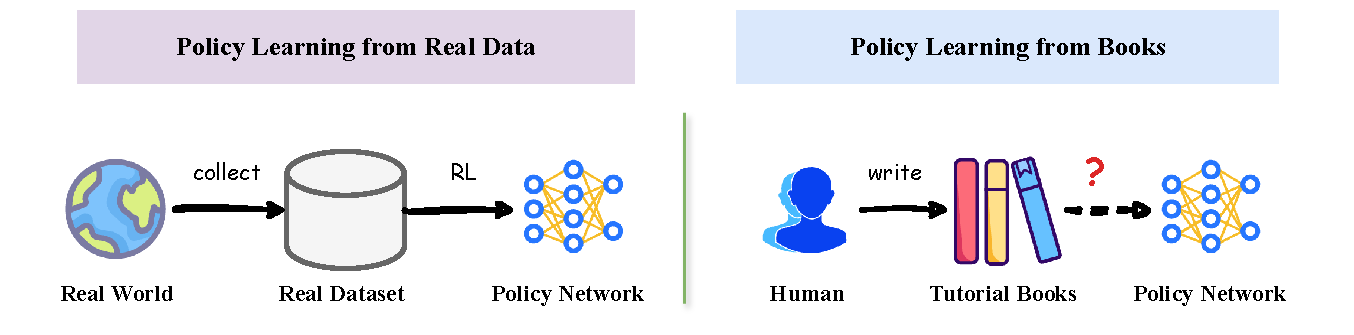
\includegraphics[width=0.75\linewidth]{fig/PER-problem.pdf}
\caption{Illustration of the relationship between aggregation rounds and the number of codes generated during PER.}
\label{fig:code_aggregation}
\end{figure}


Figure \ref{fig:code_aggregation} illustrates a clear correlation between the number of aggregation rounds in the PER method and the number of codes generated. Initially, a rapid increase in code volume is observed, indicating a high rate of new information assimilation from textual sources. As the number of aggregation rounds increases, the rate of new code generation begins to plateau, suggesting a saturation point in learning and information extraction.


The aggregation process yields codes of varying complexity, corresponding to the depth and breadth of strategies learned from the tutorial books. For instance, initial codes (Level 1) might encompass basic football tactics and rules, while more advanced codes (Level 3 and beyond) demonstrate complex strategies and gameplays, indicating a deeper understanding and integration of football tactics as extracted from the literature. These advanced codes are crucial for the agent's ability to outperform sophisticated AI opponents, as they represent a more nuanced understanding of the game.


\begin{figure*}[ht]
\centering
\includegraphics[width=0.4\linewidth]{example_code_state_embedding_correlation.png}
\caption{Example of different levels of code.}
\label{fig:code_state_embedding}
\end{figure*}


% The analysis of code aggregation in the PER model is instrumental in understanding how the agent evolves its decision-making prowess over time. By examining the progression and complexity of codes, we gain insights into the efficiency of text-based learning in reinforcement learning environments, especially in complex scenarios such as a football game. This exploration further solidifies the practicality of using large language models to distill and apply knowledge from textual sources in decision-making contexts.

\subsection{Improve Correlation between code embedding and current state embedding  [lp]}

This section examines the interplay between code embedding and current state embedding in our Policy Learning via Reading (PER) framework, with a specific focus on the impact of fine-tuning on code retrieval effectiveness. Understanding this relationship is critical for optimizing the agent's performance in extracting and utilizing knowledge from textual sources for decision-making in a simulated football environment.

\begin{figure}[ht]
\centering
\includegraphics[width=0.75\linewidth]{code_state_embedding_correlation.png}
\caption{Illustration of the correlation between code embedding and current state embedding before and after fine-tuning in the PER methodology.}
\label{fig:code_state_embedding}
\end{figure}

To demonstrate the capacity of our system to retrieve effective information from code, we compare the results before and after fine-tuning. Metrics such as accuracy or correctness in code retrieval can be used to quantify this impact. Figure \ref{fig:code_state_embedding} showcases that fine-tuning significantly enhances the alignment between code embedding and the current state embedding, indicating more accurate and relevant information retrieval post-fine-tuning.

\begin{figure}[ht]
\centering
\includegraphics[width=0.75\linewidth]{code_state_embedding_example.png}
\caption{Example.}
\label{fig:code_state_embedding}
\end{figure}

 Examining specific instances of code retrieval before and after the fine-tuning process provides practical insights. Initially, the retrieved codes may only partially align with the current state requirements, reflecting a generalized understanding. Post-fine-tuning, the codes demonstrate a high degree of specificity and relevance, indicating a more nuanced understanding and application of football strategies and tactics as per the current game state.
 
\textbf{[level 2] Comparing Different Fine-Tuning Techniques:} Different fine-tuning techniques can yield varied results in terms of code retrieval efficiency and accuracy. By comparing techniques such as supervised fine-tuning, unsupervised fine-tuning, and reinforcement learning-based fine-tuning, we can determine the most effective method for aligning code and state embeddings in our PER framework. This analysis not only enhances the performance of the agent but also contributes to the broader understanding of fine-tuning impacts in language model-based learning systems.


\subsection{Importance of the components in Imaginary-RL [xionghui]}

ablation studies among different components in offline RL.
\begin{itemize}
    \item without uncertainty estimator
    \item different implementation of offlineRL?
    \item without imaginary data.
\end{itemize}

Distribution of the dataset.

\subsection{Amount of Real Dataset Used}

[figure]

Show the relationship between the amount of offline dataset used, the imaginary dataset used, and the performance of the learned policy.

\subsection{ablation studies [ziyan-baseline]}

[figure]

\begin{itemize}
    \item PER
    \item without-RL: book-rag-$\pi$ [done]
    \item [lp]  without-book-information: GPT-data-$\pi$
\end{itemize}

\subsection{Efficiency in inference} 

\begin{figure}[ht]
\centering
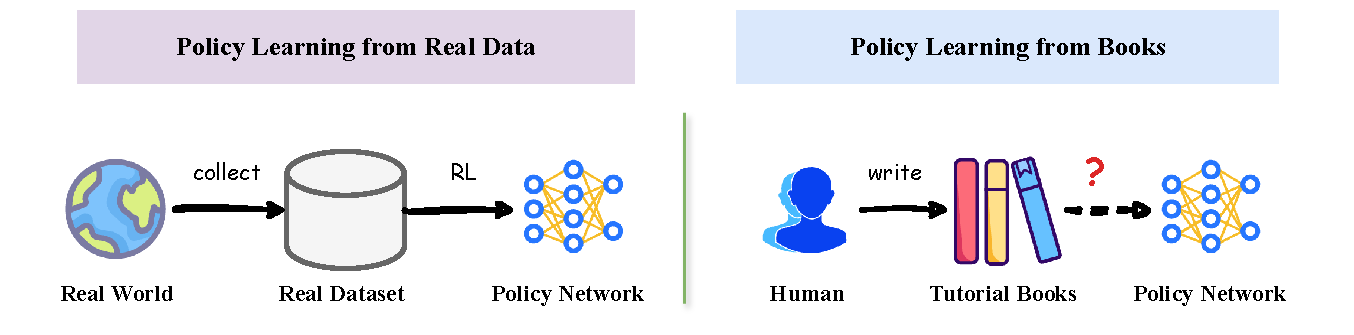
\includegraphics[width=0.75\linewidth]{fig/PER-problem.pdf}
\caption{Illustration of the time cost of one-step inference in different frameworks.}
\label{fig:code_aggregation}
\end{figure}

Show the time cost of one-step inference: compare GPT-plan, GPT-RAG, GPT, and PER.


\subsection{Case Study}
Appendix
% 1. Show some steps in imaginary data generation.

% % [figure]